% Figure 3: positioning map — producer (human->machine) x epistemic level (L1->L3)
\documentclass[tikz,border=8pt]{standalone}
% Shared preamble for SAI taxonomy standalone figures.
% Self-contained: no MetaCircle dependency; colors match the paper palette.
\usepackage{amsmath,amssymb}
\usetikzlibrary{arrows.meta}
\definecolor{MetaPurple}{HTML}{6D3BD1}
\definecolor{MetaViolet}{HTML}{9B5DE5}
\definecolor{MetaCoral}{HTML}{D76A7A}
\definecolor{MetaInk}{HTML}{16131D}
\definecolor{MetaGray}{HTML}{F4F2F7}
\definecolor{MetaMidGray}{HTML}{6E6875}
\newcommand{\Lk}{\mathcal{L}_1}
\newcommand{\Ll}{\mathcal{L}_2}
\newcommand{\Ls}{\mathcal{L}_3}
\newcommand{\Op}[1]{\textsc{#1}}
\newcommand{\universe}{\Omega}
\newcommand{\kb}{\mathcal{K}}
\newcommand{\cell}{\omega}

\begin{document}
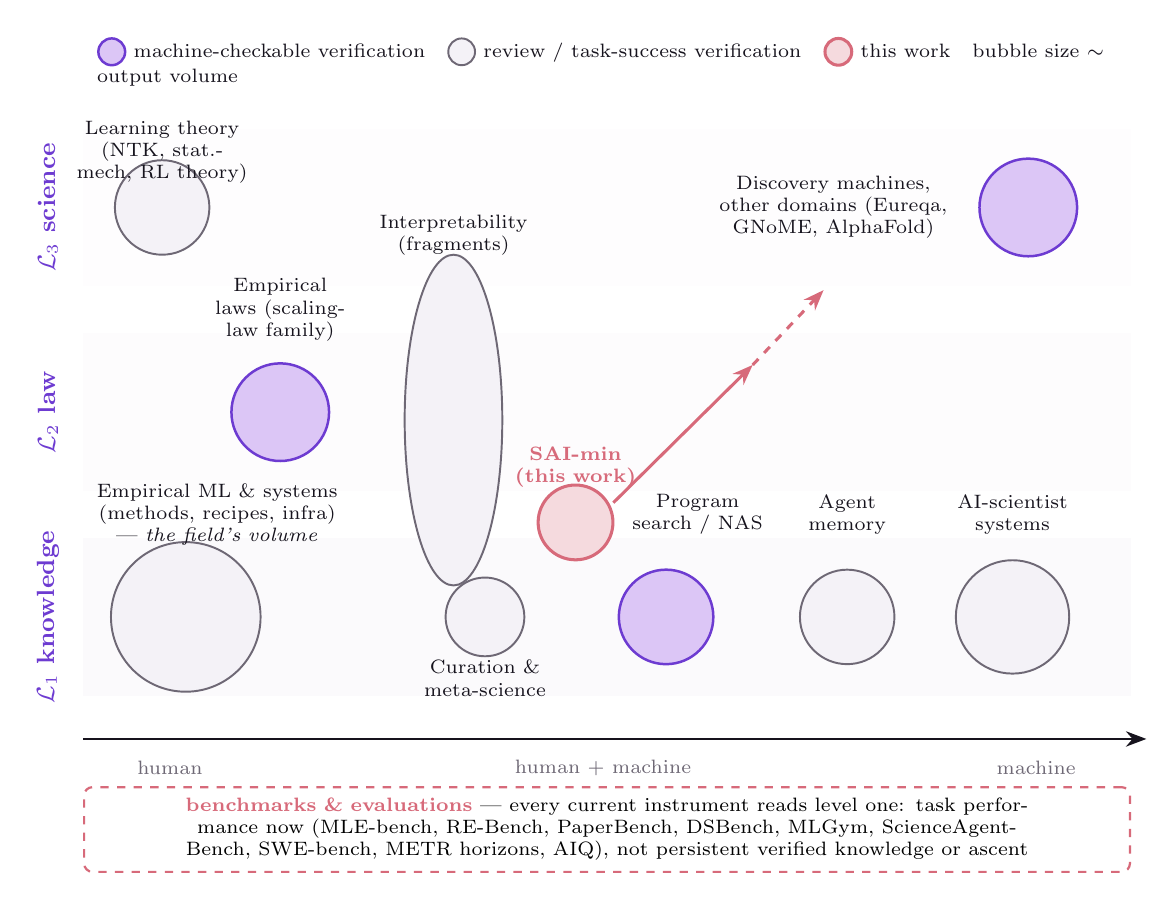
\begin{tikzpicture}[
  font=\small,
  bub/.style={circle, draw=MetaMidGray, line width=0.7pt, fill=MetaGray, inner sep=0pt},
  bubp/.style={circle, draw=MetaPurple, line width=0.9pt, fill=MetaViolet!35, inner sep=0pt},
  bubc/.style={circle, draw=MetaCoral, line width=1.1pt, fill=MetaCoral!25, inner sep=0pt},
  lab/.style={font=\scriptsize, align=center, text=MetaInk},
  band/.style={fill=MetaGray, opacity=0.35},
  arw/.style={-{Stealth[length=2.6mm]}, line width=1.1pt, MetaCoral},
]
% level bands
\fill[band] (0.9,0.7) rectangle (14.2,2.7);
\fill[band, opacity=0.22] (0.9,3.3) rectangle (14.2,5.3);
\fill[band, opacity=0.12] (0.9,5.9) rectangle (14.2,7.9);
\node[rotate=90, font=\small\bfseries, text=MetaPurple] at (0.45,1.7) {$\mathcal{L}_1$ knowledge};
\node[rotate=90, font=\small\bfseries, text=MetaPurple] at (0.45,4.3) {$\mathcal{L}_2$ law};
\node[rotate=90, font=\small\bfseries, text=MetaPurple] at (0.45,6.9) {$\mathcal{L}_3$ science};
% producer axis
\draw[-{Stealth[length=2.6mm]}, line width=0.8pt, MetaInk] (0.9,0.15) -- (14.4,0.15);
\node[font=\scriptsize, text=MetaMidGray] at (2.0,-0.22) {human};
\node[font=\scriptsize, text=MetaMidGray] at (7.5,-0.22) {human + machine};
\node[font=\scriptsize, text=MetaMidGray] at (13.0,-0.22) {machine};
% ---- L3 row ----
\node[bub, minimum size=1.2cm] at (1.9,6.9) {};
\node[lab, text width=2.6cm] at (1.9,7.6) {Learning theory (NTK, stat.-mech, RL theory)};
\node[bubp, minimum size=1.24cm] at (12.9,6.9) {};
\node[lab, text width=3.3cm, anchor=east] at (12.2,6.9) {Discovery machines, other domains (Eureqa, GNoME, AlphaFold)};
% ---- L2 row ----
\node[bubp, minimum size=1.24cm] at (3.4,4.3) {};
\node[lab, text width=2.2cm] at (3.4,5.6) {Empirical laws (scaling-law family)};
\draw[MetaMidGray, line width=0.7pt, fill=MetaGray] (5.6,4.2) ellipse (0.62cm and 2.1cm);
\node[lab, text width=2.0cm] at (5.6,6.55) {Interpretability (fragments)};
% ---- L1 row ----
\node[bub, minimum size=1.9cm] at (2.2,1.7) {};
\node[lab, text width=3.6cm] at (2.6,3.0) {Empirical ML \& systems (methods, recipes, infra) --- \emph{the field's volume}};
\node[bub, minimum size=1.0cm] at (6.0,1.7) {};
\node[lab, text width=1.9cm] at (6.0,0.92) {Curation \& meta-science};
\node[bubp, minimum size=1.2cm] at (8.3,1.7) {};
\node[lab, text width=1.9cm] at (8.7,3.0) {Program search / NAS};
\node[bub, minimum size=1.2cm] at (10.6,1.7) {};
\node[lab, text width=1.8cm] at (10.6,3.0) {Agent memory};
\node[bub, minimum size=1.44cm] at (12.7,1.7) {};
\node[lab, text width=2.0cm] at (12.7,3.0) {AI-scientist systems};
% ---- SAI-min ascent ----
\node[bubc, minimum size=0.95cm] at (7.15,2.9) {};
\node[lab, text width=1.7cm, text=MetaCoral] at (7.15,3.6) {\textbf{SAI-min (this work)}};
\draw[arw] (7.63,3.15) -- (9.4,4.9);
\draw[arw, dashed] (9.4,4.9) -- (10.3,5.85);
% legend
\node[font=\scriptsize, align=left, text=MetaInk, anchor=west, text width=13.0cm] at (0.95,8.75) {%
  \tikz[baseline=-2pt]{\node[bubp, minimum size=0.34cm]{};} machine-checkable verification\quad
  \tikz[baseline=-2pt]{\node[bub, minimum size=0.34cm]{};} review / task-success verification\quad
  \tikz[baseline=-2pt]{\node[bubc, minimum size=0.34cm]{};} this work\quad bubble size $\sim$ output volume};
% benchmark strip
\node[draw=MetaCoral, dashed, rounded corners=3pt, line width=0.8pt, font=\scriptsize, align=center, text width=13.0cm, inner sep=4pt] at (7.55,-1.0) {%
  \textbf{\textcolor{MetaCoral}{benchmarks \& evaluations}} --- every current instrument reads level one: task performance now (MLE-bench, RE-Bench, PaperBench, DSBench, MLGym, ScienceAgentBench, SWE-bench, METR horizons, AIQ), not persistent verified knowledge or ascent};
\end{tikzpicture}
\end{document}
